

\chapter{Aerial Mapping and Photogrametry} \label{chap:2}



\section{The need for mapping the land}
The first known map (actually a painting of a city) dates up to the 7th millenium BCE,\footnote{Stephanie Meece (2006). "A bird's eye view – of a leopard's spots. The Çatalhöyük 'map' and the development of cartographic representation in prehistory". Anatolian Studies. 56: 1–16. JSTOR 20065543.
}, while the oldest surviving world maps are from 9th century BCE Babylonia\footnote{ Kurt A. Raaflaub; Richard J. A. Talbert (2009). Geography and Ethnography: Perceptions of the World in Pre-Modern Societies. John Wiley & Sons. p. 147. ISBN 1-4051-9146-5.}.

In the past, maps were used mostly for localization and navigation $^{\text{[citation needed]}}$, and were made without special tools, mainly by sight. During the Age of Exploration, new tools such as the sextant and magnetic compass helped improve accuracy, while remaining as a navigational tool.

On the last centuries, maps began being used to precisely map properties, natural landscapes, and cities. Mapping properties, for example, requires high dimensional accuracy, hard to get with regular tools. This is usually the job of land surveyors, professionals who use a multitude of tools, such as total stations, robotic total stations, GPS receivers, retroreflectors, 3D scanners, radios, handheld tablets, digital levels, subsurface locators, drones, GIS, and surveying software.


\section{Aerial Mapping}
Aerial mapping consists of using photographs taken from the air, usually with the camera facing straight downwards, correcting the perspective transformation, and assembling them into an orthomosaic, as seen on Figure \ref{fig:orthomosaic}.

\begin{figure}
\centering
  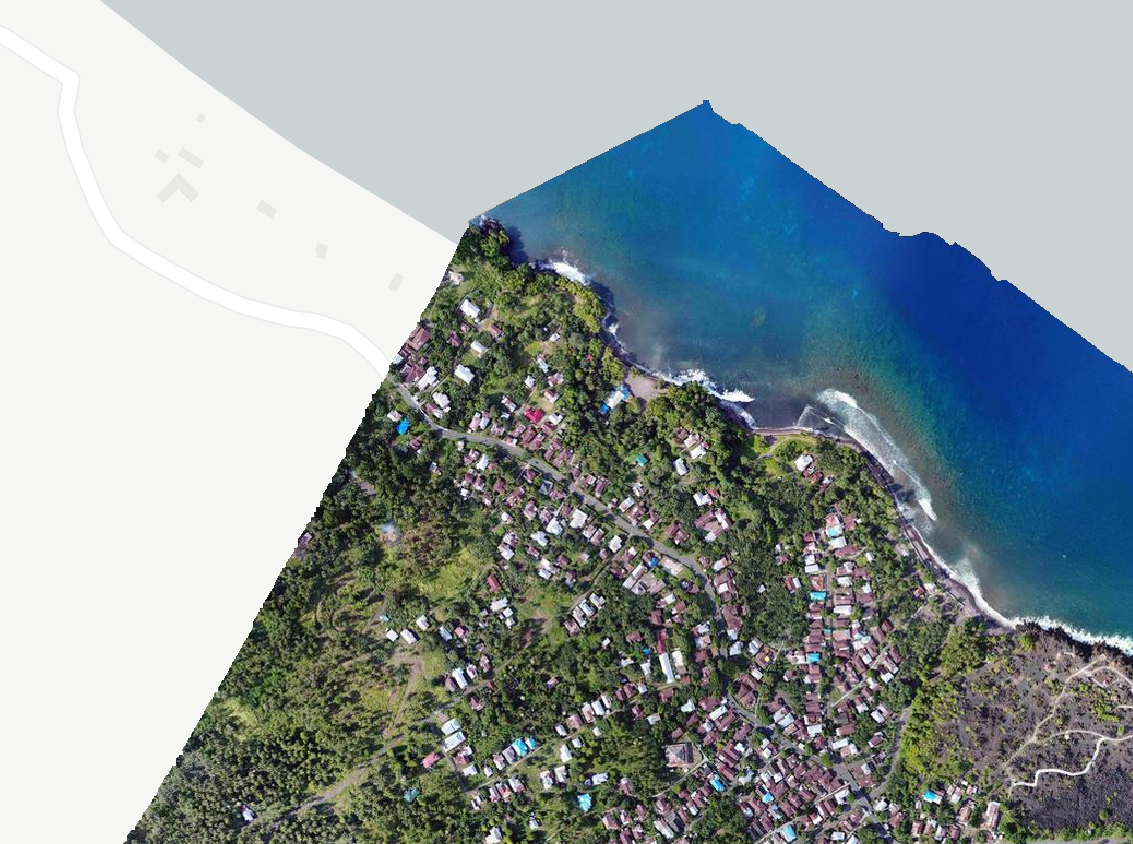
\includegraphics[width=\linewidth]{figs/orthomosaic.png}
  \caption{Orthomosaic. source: Indonesian Redcross/OpenAerialMap}
  \label{fig:orthomosaic}
\end{figure}


\section{Aerophotogrammetry}

Aerophotogrammetry takes the job on step further. By knowing the cameras lens intrinsics, software are capable of matching a number of pictures, detecting features on the environment, and locating the point used to take each of the pictures. With this information, it's possible to rebuild in 3D most of the environments, enabling the operator to interact with the area as a 3D mesh.
By using precise GPS information(such as RTK/PPK data, or total stations) or known landmarks, it's possible to accurately measure distances, areas, volumes, angles and elevations, simplifying the surveyors' job.

Aerophotogrametry can also rebuild in 3D buildings and other structures, 